\section{Large worlds of mathematical structures}
Based on sets and functions.
\subsection{Monoids and Homomorphisms}
Suppose some function $f: \mathbb{N} \rightarrow \mathbb{Z}$ and $f(n)=n$. This
function $f$ respects addition in the following sense.
\begin{align*}
	f(m+n) = f(m) + f(n)
\end{align*}
We can add $m+n$ first and then map it via $f$, or we can first map $m, n$ via
$f$, and then add them.
\begin{figure}[H]
	\begin{center}
		\documentclass{standalone}
\usepackage{tikz}
\begin{document}
\begin{tikzpicture}
	\node {$f$}
	child {node {$+$}
			child {node {$m$}}
			child {node {$n$}}
		};
\end{tikzpicture}
\begin{tikzpicture}
	\node {$+$}
	child {node {$f$}
			child {node {$m$}}
		}
	child {node {$f$}
			child {node {$n$}}
		};
\end{tikzpicture}
\end{document}

	\end{center}
	\caption{Homomorphism tree representation}
\end{figure}

\begin{ttta}
	Another possible function $f: \mathbb{N} \rightarrow \mathbb{Z}$ is given by
	$f(n) = 2n$. See if you can check that this also satisfies the above condition
	$f(m+n) = f(m) + f(n)$.
	\begin{align*}
		f(m+n) = & f(m) + f(n) \\
		2(m+n) = & 2(m) + 2(n) \\
		2(m+n) = & 2(m+n)      \\
		m+n =    & m+n
	\end{align*}
	Thus we have shown that $f$ respects addition.
\end{ttta}

\begin{ttta}
	Show that this function
	\[
		f=\set{(0, 0), (1, 1), (2, -1), (3, 2), (4, -2), (5, 3), (6, -3), \dots}
	\]
	does not respect addition.
	\begin{align*}
		f(1+3) =      & f(4)  \\
		=             & -2    \\
		f(1) + f(3) = & 1 + 2 \\
		=             & 3     \\
		3 \neq        & -2    \\
	\end{align*}
\end{ttta}

\begin{ttta}
	Mapping into the integers is special because it turns out that respecting
	addition forces a function to respect the identity. Prove it.
\end{ttta}
\begin{figure}[H]
	\begin{center}
		\documentclass{standalone}
\usepackage{tikz}
\begin{document}
\begin{tikzpicture}
	\node {$f$}
	child {node {$+$}
			child {node {$0$}}
			child {node {$n$}}
		};
\end{tikzpicture}
\begin{tikzpicture}
	\node {$f$}
	child {node {$+$}
			child {node {$n$}}
		};
\end{tikzpicture}
\begin{tikzpicture}
	\node {$+$}
	child {node {$f$}
			child {node {$0$}}
		}
	child {node {$f$}
			child {node {$n$}}
		};
\end{tikzpicture}
\end{document}

	\end{center}
\end{figure}
\begin{proofitem}
	\item To respect addition, a function $f$ must satisfy the following equation $f(m+n) =
		f(m)+f(n)$.  Suppose that $f$ does respect addition and use that to show respecting addition
	implies that $f$ also respects the identity.
	\begin{align*}
		f(m+n) = & f(0 +n)     &  & m=0                         \\
		f(0+n) = & f(0) + f(n) &  & \text{homomorphism}         \\
		f(n) =   & f(0) + f(n)                                  \\
		f(0) =   & 0           &  & f\;\text{respects identity}
	\end{align*}
\end{proofitem}

\begin{figure}[H]
	\begin{center}
		\documentclass{standalone}
\usepackage{tikz}
\begin{document}
\begin{tikzpicture}
  \node {$f$}
    child {node {$\circ$}
      child {node {$x$}}
      child {node {$y$}}
    };
\end{tikzpicture}
\begin{tikzpicture}
  \node {$\circ$}
    child {node {$f$}
      child {node {$x$}}
    }
    child {node {$f$}
      child {node {$y$}}
    };
\end{tikzpicture}
\end{document}

	\end{center}
\end{figure}
\begin{definition}
	Let $A$ and $B$ be monoids, and write the identity as $1$ and the
	binary operation as $\circ$ in each case. Then a monoid homomorphism from A to
	B is a function $f:A\rightarrow B$ on the underlying sets, such that
	\begin{align*}
		\forall x, y \in A, f(x \circ y) & = f(x) \circ f(y) &  & f\text{ respects }\circ    \\
		f(1)                             & =1                &  & f\text{ respects identity}
	\end{align*}
\end{definition}

\subsubsection{Example 1}
\begin{proofitem}
	\item Let $M\subseteq\mathbb{Z}_3=\set{0, 1, 2}$. The monoid is $(M, +_3, 0)$.
	\item Let $N\subseteq\mathbb{Z}=\set{2, 3, 7}$.
	The monoid is $(N, \min, 7)$.
	\item Lef $f: M \rightarrow N\subseteq \mathbb{Z}_3\times\mathbb{Z}=\set{(0, 7),
			(1, 2), (2, 3)}$.
	\begin{align*}
		f(x\circ y) & = f(x)\circ f(y)  \\
		f(0 +_3 3)  & = f(0)`\min` f(3) \\
		f(3)        & = 7`\min` 1       \\
		1           & = 1               \\
		f(1 +_3 2)  & = f(1)`\min` f(2) \\
		f(0)        & = 2`\min` 1       \\
		7           & \neq 1
	\end{align*}
	Thus $f$ is not a monoid homomorphism.
\end{proofitem}
\clearpage
\begin{ttta}
	What needs to be checked to show that monoids and their homomorphisms form
	a category?
\end{ttta}
\begin{proofitem}
	\item To check that monoids and their homomorphisms form a category, we
	must show that the category, call it \textbf{Mnd}, respects identity
	and composition. Showing identity and associativity where objects are sets
	and morphisms are functions is trivial because the universal existence of
	the identity function and because function composition guarantees
	associativity. Because we are declaring that all objects of \textbf{Mnd}
	are monoids, we must check that the morphisms between objects preserve
	structure, meaning that the morphisms are homomorphisms.

	\item Let $f, g$ be monoid homomorphisms, ie they are arrows between objects in the category \textbf{Mnd}.
	\item Let $\circ$ be a binary composition operation on arrows.
	\item Let $\ast$ be a binary composition operation on monoidal elements.
	\setcounter{equation}{0}
	\begin{align*}
		(g\circ f)(x\ast y) & = g(f(x\ast y))                    &  & \text{def.\;of }\circ         \\
		                    & = g(f(x) \ast f(y))                &  & f\text{ respects }\ast        \\
		                    & = g(f(x)) \ast g(f(y))             &  & g\text{ respects }\ast        \\
		                    & = (g\circ f)(x) \ast (g\circ f)(y) &  & g\circ f\text{ respects }\ast \\
		(g\circ f)(1)       & = g(f(1))                          &  & f\text{ respects }1           \\
		                    & = g(1)                             &  & g \text{ respects }1          \\
		                    & = 1                                &  & g \circ f\text{ respects }1
	\end{align*}
\end{proofitem}
\begin{figure}[H]
	\begin{center}
		\documentclass[border=0.2cm]{standalone}
\usepackage{tikz}
\usepackage{titlesec}
\usepackage{float}
\usepackage{standalone}
\usepackage{tikzit}
\usetikzlibrary{automata, arrows.meta, positioning}
\usetikzlibrary{arrows.meta, positioning}
\input{figures/sample-02.tikzstyles}

\begin{document}
\begin{tikzpicture}[scale=1.0]
	\begin{pgfonlayer}{nodelayer}
		\node [style=object] (0) at (0, 0) {$M_A$};
		\node [style=object] (1) at (4, 0) {$M_B$};
		\node [style=object] (2) at (8, 0) {$M_C$};
	\end{pgfonlayer}
	\begin{pgfonlayer}{edgelayer}
		\path [-stealth, thick]
		(0) edge node[above] {$f$}   (1)
		(1) edge node[above] {$g$}   (2)
		(0) edge [out=210, in=240, looseness=8, below]  node {$x$}(0)
		(0) edge [out=330, in=300, looseness=8, below]  node {$y$}(0)
		(0) edge [loop above] node[above] {$x\ast y$}(0)
		(1) edge [out=210, in=240, looseness=8, below]  node {$x$}(1)
		(1) edge [out=330, in=300, looseness=8, below]  node {$y$}(1)
		(1) edge [loop above] node[above] {$f(x\ast y)$}(1)
		(2) edge [out=210, in=240, looseness=8, below]  node {$x$}(2)
		(2) edge [out=330, in=300, looseness=8, below]  node {$y$}(2)
		(2) edge [loop above] node[above] {$(g\circ f)(x\ast y)$}(2) ;
	\end{pgfonlayer}
\end{tikzpicture}
\end{document}

	\end{center}
	\caption{Monoid Category $\mathbf{Mnd}$}
\end{figure}
\subsection{Groups}

\begin{ttta}
	Define group homomorphisms as a function respecting the group structure. When
	dealing with groups, it is redundant to ask for the identity to be preserved.
	It’s also redundant to ask for the inverses to be preserved. Prove this.
\end{ttta}
\begin{proofitem}
	\item The properties needed for a function to be a group homomorphism are the
	preservation of group properties, namely: identity, invertibility, and
	preservation of the binary operation.
	\item Suppose $f: G \rightarrow H$ is a homomorphism between groups $G$ and $H$.
	We will show that the if $f$ preserves the binary operation, $f$ also
	preserves the identity.
	\begin{align*}
		f(1) =             & f(a\circ a^{-1})    &  & \text{def.\;of\;}1         \\
		=                  & f(a)\circ f(a^{-1}) &  & f\;\text{preserves}\;\circ \\
		=                  & 1                   &  & \text{def.\ of inverse}    \\
		f(a\circ a^{-1}) = & f(a)\circ f(a^{-1}) &  & f\;\text{preserves}\;\circ \\
		f(1) =             & 1                   &  & f\;\text{preserves}\;^{-1} \\
	\end{align*}
\end{proofitem}

\begin{ttta}
	Do we have to check anything else to show that groups and group homomorphisms form a category?
\end{ttta}
Because groups are monoids with an extra property, there is nothing to check
because monoids already form a cateogry. In other words, the monoidal nature of
a group is sufficient to show unitality and associativity for a category
$\mathbf{Grp}$ created from some set that is also a group.

\subsection{Posets}
\begin{ttta}
	Create a definition of an order-preserving function for posets in general by
	analogy with the structure-preserving maps we've seen already.
\end{ttta}
\begin{proofitem}
	\item Let $f:P\rightarrow Q$ be some function between two posets $P$ and $Q$.
	Because $P$ and $Q$ are posets, we know that individually they both have the
	properties reflexivity, transitivity, and antisymmetry. For $f$ to be order
	preserving, the only condition on $f$ is
	\begin{align*}
		x\geq_P y \implies f(x)\geq_Q f(y)
	\end{align*}
\end{proofitem}

\begin{ttta}
	Do we have to check anything to show that we have a category of posets and order-preserving functions?
\end{ttta}
\begin{proofitem}
	\item The arrows between posets are functions. It is always possible to create
	identity functions and function composition (see\footnote{see TTTA\ref{ttta:function-forms-category}}), and these properties
	automatically imply the required category properties---unitality and associativity.
	\item Therefore the only thing to check is that the functions preserve ordering
	between the posets.
\end{proofitem}
For arrows $g$ and $f$ in the category of $\mathbf{Poset}$ to preserve
structure, the following must be true.
\begin{align*}
	x \geq y & \implies f(x) \geq f(y)                   \\
	         & \implies g(f(x)) \geq g(f(y))             \\
	         & \implies (g\circ f)(x) \geq (g\circ f)(y) \\
\end{align*}
\begin{figure}[H]
	\begin{center}
		\documentclass[border=0.2cm]{standalone}
\usepackage{tikz}
\usepackage{titlesec}
\usepackage{float}
\usepackage{standalone}
\usepackage{tikzit}
\usetikzlibrary{automata, arrows.meta, positioning}
\usetikzlibrary{arrows.meta, positioning}
\input{figures/sample-02.tikzstyles}
\begin{document}

\begin{tikzpicture}
	\begin{pgfonlayer}{nodelayer}
		\node [style=object] (0) at (0, 0) {$P_A$};
		\node [style=object] (1) at (4.5, 0) {$P_B$};
		\node [style=object] (2) at (9, 0) {$P_C$};
	\end{pgfonlayer}
	\begin{pgfonlayer}{edgelayer}
		\path [-stealth, thick]
		(0) edge node[above] {$f$}   (1)
		(1) edge node[above] {$g$}   (2)
		(0) edge [out=30, in=60, looseness=8, below]  node[above] {$1$}(0)
		(0) edge [out=120, in=150, looseness=8, below] node[above] {$x\ast y$}(0)
		(0) edge [out=210, in=240, looseness=8, below]  node[below] {$x$}(0)
		(0) edge [out=300, in=330, looseness=8, below]  node[below] {$y$}(0)
		(1) edge [out=30, in=60, looseness=8, below]  node[above] {$f(1)$}(1)
		(1) edge [out=120, in=150, looseness=8, below] node[above] {$f(x\ast y$)}(1)
		(1) edge [out=210, in=240, looseness=8, below]  node[below] {$f(x)$}(1)
		(1) edge [out=300, in=330, looseness=8, below]  node[below] {$f(y)$}(1)
		(2) edge [out=30, in=60, looseness=8, below]  node[above, xshift=1cm] {$(g\circ f)(1)$}(2)
		(2) edge [out=120, in=150, looseness=8, below] node[xshift=-0.4cm,above] {$(g\circ f)(x\ast y$)}(2)
		(2) edge [out=210, in=240, looseness=8, below]  node[xshift=-0.5cm, below] {$(g\circ f)(x)$}(2)
		(2) edge [out=300, in=330, looseness=8, below]  node[xshift=0.5cm, below] {$(g\circ f)(y)$}(2)
		;
	\end{pgfonlayer}
\end{tikzpicture}

\end{document}

	\end{center}
	\caption{Poset Category $\mathbf{Poset}$}
\end{figure}

\begin{ttta}
	Think again about the poset of factors of 42.
	Observe that $6 < 7$ but 6 is higher than 7 in this diagram. What two orderings
	are we considering on the same set of numbers here, and what map is it that is
	not order-preserving?
\end{ttta}
\begin{figure}[H]
	\begin{center}
		\documentclass[border=0.2cm]{standalone}
\usepackage{tikz}
\usepackage{titlesec}
\usepackage{float}
\usepackage{standalone}
\usepackage{tikzit}
\usetikzlibrary{automata, arrows.meta, positioning}
\usetikzlibrary{arrows.meta, positioning}
\input{figures/sample-02.tikzstyles}

\begin{document}
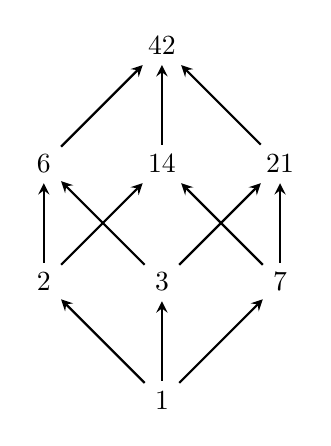
\begin{tikzpicture}[->, >=stealth, thick]
	\node (1) at (3,0) {$1$};
	\node (2) at (1.5,1.5) {$2$};
	\node (3) at (3,1.5) {$3$};
	\node (5) at (4.5,1.5) {$7$};
	\node (6) at (1.5,3) {$6$};
	\node (10) at (3,3) {$14$};
	\node (15) at (4.5,3) {$21$};
	\node (30) at (3,4.5) {$42$};
	\draw (1) -- (2);
	\draw (1) -- (3);
	\draw (1) -- (5);
	\draw (2) -- (6);
	\draw (2) -- (10);
	\draw (3) -- (6);
	\draw (3) -- (15);
	\draw (5) -- (10);
	\draw (5) -- (15);
	\draw (6) -- (30);
	\draw (10) -- (30);
	\draw (15) -- (30);
\end{tikzpicture}
\end{document}

	\end{center}
	\caption{42-factor lattice}
\end{figure}
\begin{proofitem}
	\item Let $S=\set{1,2, 3, 6, 7, 14, 21, 42}\subset \mathbb{N}$.
	\item One order is $\geq$ as defined on $\mathbb{N}$.
	The other order is divides $\mid$, as in $a\mid b$---for example $6\mid 12$.
	Both orders are reflexive, anti-symmetric, and transitive, as required by
	definition.
	\item Let us consider the map $f:\mathbb{N}\rightarrow\mathbb{N}$, where $f=+1$.
	For the ordering $\geq$, $f$ preserves ordering.
	\begin{align*}
		f(x \geq y) = & f(x) \geq f(y) \\
		=             & x+1 \geq y+1   \\
		=             & x \geq y
	\end{align*}
	Now we will show that $f$ does not preserve ordering on $\mid$ by
	counter-example.
	\begin{align*}
		f(x \mid y) =  & f(x) \mid f(y)  &  & \text{Let }x=7, y=14 \\
		f(7 \mid 14) = & f(7) \mid f(14)                           \\
		\neq           & 8 \mid 15
	\end{align*}
	Thus we have shown that $\mid$ does not preserve ordering.
\end{proofitem}

\subsection{Categories}
\begin{ttta}
	Think of a sensible starting point for a definition of a morphism of
	categories $F: \mathbb{C} \longrightarrow \mathbb{D}$. It should map objects to
	objects and arrows to arrows, but if we start with an arrow $f: x \rightarrow
		y\in\mathbb{C}$ what should the source and target of $F(f)$ be in
	$\mathbb{D}$?
\end{ttta}
\begin{proofitem}
	\item
	\begin{align*}
		f\in \mathbb{C}    & : x \rightarrow y       \\
		F(f)\in \mathbb{D} & : F(x) \rightarrow F(y)
	\end{align*}
\end{proofitem}

\begin{definition}
	A category is called small if its objects form a set (not a large collection)
	and its morphisms also form a set.
\end{definition}
\begin{ttta}
	Come up with the definition of a morphism between categories, starting with the
	action of $F$ on objects and arrows. Then proceed by making sure it is
	structure-preserving. To do this, you need to be clear what the structure of a
	category is: identities and composition. Once you've done this, can you check
	that this gives us a category of small categories and all morphisms between
	them.
\end{ttta}
\begin{figure}[H]
	\begin{center}
		\documentclass[border=0.2cm]{standalone}
\usepackage{tikz}
\usepackage{titlesec}
\usepackage{float}
\usepackage{standalone}
\usepackage{tikzit}
\usetikzlibrary{automata, arrows.meta, positioning}
\usetikzlibrary{arrows.meta, positioning}
\input{figures/sample-02.tikzstyles}

\begin{document}
\begin{tikzpicture}
	\begin{pgfonlayer}{nodelayer}
		\node [style=object] (0) at (0, 0) {$\mathbb{C}$};
		\node [style=object] (1) at (4.5, 0) {$\mathbb{D}$};
		\node [style=object] (2) at (9, 0) {$\mathbb{E}$};
	\end{pgfonlayer}
	\begin{pgfonlayer}{edgelayer}
		\path [-stealth, thick]
		(0) edge node[above] {$F$}   (1)
		(1) edge node[above] {$G$}   (2)
		(0) edge [out=30, in=60, looseness=8, below]  node[above] {$1$}(0)
		(0) edge [out=120, in=150, looseness=8, below] node[above] {$x\ast y$}(0)
		(0) edge [out=210, in=240, looseness=8, below]  node[below] {$x$}(0)
		(0) edge [out=300, in=330, looseness=8, below]  node[below] {$y$}(0)
		(1) edge [out=30, in=60, looseness=8, below]  node[above] {$F(1)$}(1)
		(1) edge [out=120, in=150, looseness=8, below] node[above] {$F(x\ast y$)}(1)
		(1) edge [out=210, in=240, looseness=8, below]  node[below] {$F(x)$}(1)
		(1) edge [out=300, in=330, looseness=8, below]  node[below] {$F(y)$}(1)
		(2) edge [out=30, in=60, looseness=8, below]  node[above, xshift=1cm] {$(G\circ F)(1)$}(2)
		(2) edge [out=120, in=150, looseness=8, below] node[xshift=-0.4cm,above] {$(G\circ F)(x\ast y$)}(2)
		(2) edge [out=210, in=240, looseness=8, below]  node[xshift=-0.5cm, below] {$(G\circ F)(x)$}(2)
		(2) edge [out=300, in=330, looseness=8, below]  node[xshift=0.5cm, below] {$(G\circ F)(y)$}(2)
		;
	\end{pgfonlayer}
\end{tikzpicture}
\end{document}

	\end{center}
	\caption{Category and Functor}
\end{figure}
\begin{definition}
	A morphism between categories $\mathbb{C}$ and $\mathbb{D}$ needs to map all
	data elements in $\mathbb{C}$ to $\mathbb{D}$. The data elements consist of
	arrows and objects.
	By definition, all the objects in $\mathbb{D}$ will have an identity arrow, and
	any arrows $f:a\rightarrow b, g:b\rightarrow c\in\mathbb{D}$ will compose
	such that $g\circ f:a\rightarrow c$.
\end{definition}
\begin{proofitem}
	\item $F$ must preserve identity-structure such that
	\begin{align*}
		f \circ 1_x =    & f                 \\
		F(f \circ 1_x) = & F(f) \circ F(1_x) \\
		=                & F(f) \circ 1_y    \\
		=                & F(f)              \\
		1 \circ f =      & f                 \\
		F(1 \circ f) =   & F(1) \circ F(f)   \\
		=                & 1 \circ F(f)      \\
		=                & F(f)
	\end{align*}
	For an arrow $f: x \rightarrow y$ in category $\mathbb{C}$.
	\begin{align*}
		f \circ 1_x =       & f        &  & \text{Identity Law in Category C}    \\
		F(f \circ 1_x) =    & F(f)     &  & \text{Applying the Functor F}        \\
		F(f) \circ F(1_x) = & F(f)     &  & \text{Functor Preserves Composition} \\
		F(1_x) =            & 1_{F(x)}
	\end{align*}
	incomplete\ldots wait till the functor chapter
\end{proofitem}
